\section{Procesadores Superescalares}

Una implementación superescalar de la arquitectura de un procesador es aquella en la que las instrucciones comunes pueden iniciar su ejecución simultáneamente y ejecutarse de manera independiente. Estas implementaciones plantean complejos problemas de diseño relacionados con el cauce de instrucciones.

Lo esencial del enfoque superescalar es su habilidad para ejecutar instrucciones en diferentes cauces de manera independiente y concurrente. El concepto puede llevarse más lejos permitiendo que las instrucciones se ejecuten en un orden diferente al del programa. 

\subsection{Superescalar frente a supersegmentado}

La supersegmentación aprovecha el hecho de que muchas etapas del cauce realizan tareas que requieren menos de medio ciclo de reloj. De este modo, doblando la velocidad de reloj interna se permite la realización de dos tareas en un ciclo de reloj externo.

Las etapas macro se dividen en el cauce segmentado en sub-etapas más pequeñas y se transmiten los datos a la mayor velocidad del ciclo de reloj.

El enfoque supersegmentado aumenta el grado de paralelismo e incrementa la aceleración percibida.

El enfoque superescalar permite llevar a cabo más de una instrucción de manera simultánea. Conlleva la duplicación de algunas o todas las partes de la CPU/ALU.\@ Debe ser capaz de captar múltiples instrucciones al mismo tiempo. Ejecutar sumas y multiplicaciones simultáneamente. Ejecutar carga/almacenamiento, mientras se lleva a cabo una operación en ALU.\@ El grado de paralelismo y, por tanto, la aceleración de la máquina aumenta, ya que se ejecutan más instrucciones en paralelo.

\begin{figure}[H]
  \centering
  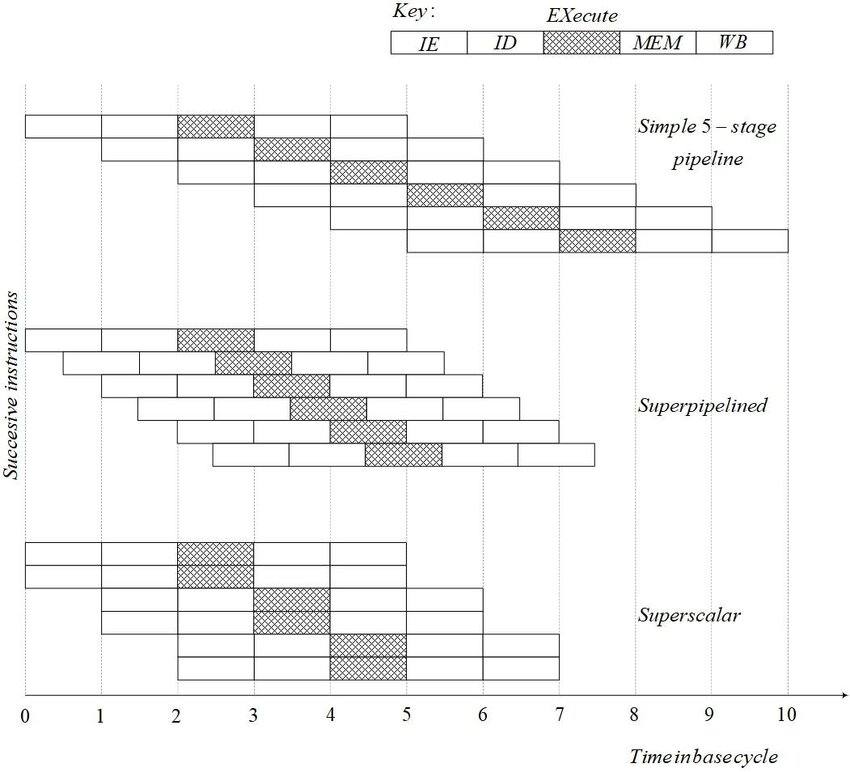
\includegraphics[width=0.5\textwidth]{SSvsSP.png}
  \caption{Superescalar contra Supersegmentado.}
\end{figure}

\subsection*{Limitaciones}

La aproximación superescalar depende de la habilidad para ejecutar múltiples instrucciones en paralelo. La expresión \textbf{paralelismo en las instrucciones} se refiere al grado en el que, en promedio, las instrucciones de un programa se pueden ejecutar en paralelo. Para maximizar el paralelismo en las instrucciones, se puede usar una combinación de optimizaciones realizadas por el compilador y de técnicas de hardware. Las principales limitaciones son:

\begin{itemize}
  \item \textbf{Dependencia de datos verdadera:} es cuando una instrucción necesita el dato producido por la primera instrucción. Si no hay dependencias, se puede captar y ejecutar dos instrucciones en paralelo. En caso de que exista esta dependencia de datos entre la primera y la segunda instrucción, se retrasa la segunda instrucción tantos ciclos de reloj como sea necesario para eliminar la dependencia.
  \item \textbf{Dependencia relativa al procedimiento:} la presencia de saltos en una secuencia de instrucciones complica el funcionamiento del cauce. Las instrucciones que siguen a una bifurcación tienen una dependencia relativa al procedimiento en ese bifurcación y no pueden ejecutarse hasta que se ejecute el salto.
  \item \textbf{Conflicto en los recursos:} Un conflicto en un recurso es una pugna de dos o más instrucciones por el mismo recurso al mismo tiempo. Desde el punto de vista del cauce segmentado, un conflicto en los recursos presenta el mismo comportamiento que una dependencia de datos. No obstante, hay algunas diferencias. Los conflictos en los recursos pueden superarse duplicando estos. Además, cuando una operación tarda mucho tiempo en finalizar, los conflictos en los recursos se pueden minimizar segmentando la unidad funcional apropiada.
  \item \textbf{Dependencia de salida.}
  \item \textbf{Antidependencia:} la restricción es similar a la de la dependencia verdadera pero a la inversa. En lugar e que la primera instrucción produzca un valor que usa la segunda instrucción, la segunda instrucción destruye un valor que utiliza la primera instrucción.
\end{itemize}

\subsection{Cuestiones relacionadas con el diseño}

\subsubsection*{Paralelismo en las instrucciones y paralelismo de la máquina}

El \textbf{paralelismo en las instrucciones} existe cuando las instrucciones de una secuencia son independientes y por tanto pueden ejecutarse en paralelo solapándose.

El paralelismo en las instrucciones depende de la frecuencia de dependencias de datos verdaderas y dependencias relativas al procedimiento que haya en el código. Estos factores dependen a su vez de la arquitectura del repertorio de instrucciones y de la aplicación.

El \textbf{paralelismo de la máquina} es una medida de la capacidad del procesador pra sacar partido al paralelismo en las instrucciones. El paralelismo de maquina depende del número de instrucciones que pueden captarse y ejecutarse al mismo tiempo y de la velocidad y sofisticación de los mecanismos que usa el procesador para localizar instrucciones independientes.

\subsubsection*{Políticas de emisión de instrucciones}

Se utiliza el término \textbf{emisión de instrucciones} para referirse al proceso de iniciar la ejecución de instrucciones en las unidades funcionales del procesador y el término \textbf{política de emisión de instrucciones} para referirse al protocolo usado para emitir instrucciones. 

El procesador intenta localizar instrucciones más allá del punto de ejecución en curso que puedan introducirse en el cauce y ejecutarse. Hay tres ordenaciones importantes:

\begin{itemize}
  \item El orden en que se captan las instrucciones.
  \item El orden en que se ejecutan las instrucciones.
  \item El orden en que las instrucciones actualizan los contenidos de los registros y de las posiciones de memoria.
\end{itemize}

Cuanto más sofisticado sea el procesador, menos limitado estará por la estrecha relación entre estas ordenaciones. Para optimizar la utilización de los diversos elementos del cauce, el procesador tendrá que alterar uno o más de estos órdenes con respecto al orden que se encontraría en una ejecución secuencial estricta. La única restricción que tiene el procesador es que el resultado debe ser correcto. De este modo, el procesador tiene que acomodar las diversas dependencias y conflictos discutido antes.

Podemos agrupar las políticas de emisión de instrucciones de los procesadores superescalares en las siguientes categorías:

\begin{itemize}
  \item \textbf{Emisión en orden y finalización en orden:} es la política de emisión más sencilla. Consiste en emitir instrucciones en el orden exacto en que lo haría una ejecución secuencial y escribir los resultados en ese mismo orden. Ni siquiera los cauces escalares siguen una política tan ingenua. No obstante, es útil considerar esta política como base con la cual comparar otras aproximaciones más sofisticadas.
  \item \textbf{Emisión en orden y finalización desordenada:} la finalización desordenada se usa en los procesadores RISC escalares para mejorar la velocidad de las instrucciones que necesitan ciclos. Con finalización desordenada, puede haber cualquier número de instrucciones en la etapa de ejecución en un momento dado, hasta alcanzar el máximo grado de paralelismo e la máquina ocupando todas la unidades funcionales. La emisión de instrucciones se para cuando hay una pugna por un recurso, una dependencia de datos o una dependencia relativa al procedimiento. Surge la \textbf{dependencia de salida}.
  \item \textbf{Emisión desordenada y finalización desordenada:} para permitir la emisión desordenada, es necesario desacoplar las etapas del cauce de decodificación y ejecución. Esto se hace mediante un buffer llamado \textbf{ventana de instrucciones}. Con esta organización, cuando un procesador termina de decodificar una instrucción, la coloca en la ventada de instrucciones. Mientras el buffer no se llene, el procesador puede continuar captando y decodificando nuevas instrucciones. Cuando una unidad funcional de la etapa de ejecución queda disponible, se puede emitir una instrucción desde la ventana de instrucciones a la etapa de ejecución. La única restricción es que el programa funcione correctamente. Por esta política surge el termino \textbf{antidependencia}.
\end{itemize}

\subsubsection*{Renombramiento de registros}

Cuando varias instrucciones compiten por el uso de los mismos registros, generando restricciones en el cauce que reducen las prestaciones. Un método para hacer frente a este tipo de conflictos de almacenamiento se basa en una solución tradicional para los conflictos en los recursos: la duplicación de recursos.

Con el \textbf{renombramiento de registros}, el hardware del procesador asigna dinámicamente los registros, que están asociados con los valores que necesitan las instrucciones en diversos instantes de tiempo. Cuando se crea un nuevo valor de registro, se asigna un nuevo registro para ese valor. Las instrucciones posteriores que accedan a ese valor como operando fuente en ese registro tienen que sufrir un proceso de renombramiento: las referencias a registros de esas instrucciones han de revisarse para referenciar el registro que contiene el valor que se necesita. 

\subsubsection*{Ejecución superescalar}

El proceso de captación de instrucciones, que incluye la predicción de saltos, se usa para formar un flujo dinámico de instrucciones. Se examinan las dependencias de este flujo, y el procesador puede eliminar las que sean artificiales. En esta ventana, las instrucciones ya no forman un flujo secuencial sino que están estructuradas de acuerdo a sus dependencias de dots verdaderas. El procesador lleva a cabo la etapa de ejecución de cada instrucción en un orden determinado por las dependencias de datos verdaderas y la disponibilidad de los recursos hardware. Por último, las instrucciones se vuelven a poner conceptualmente en un orden secuencial y sus resultados se almacenan.

\begin{figure}
  \centering
  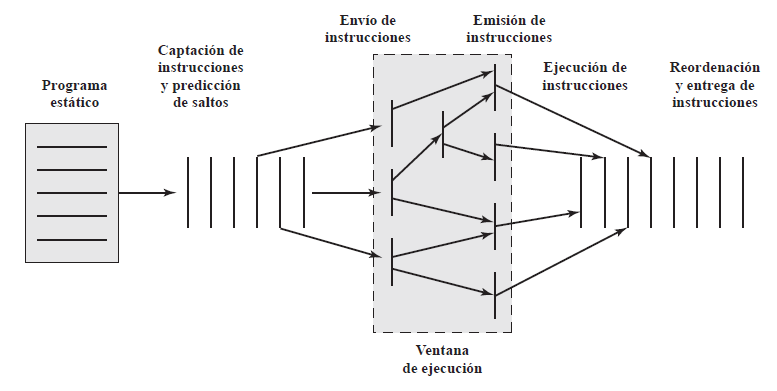
\includegraphics[width=0.7\textwidth]{ProcesamientoSE.png}
  \caption{Representación conceptual del procesamiento superescalar}
\end{figure}

\subsubsection*{Implementación superescalar}

\begin{itemize}
  \item Estrategias de captación simultánea de múltiples instrucciones.
  \item Lógica para determinar dependencias verdaderas entre valores de registros y mecanismos para comunicar esos valores.
  \item Mecanismos para iniciar o emitir múltiples instrucciones en paralelo.
  \item Recursos para la ejecución en paralelo de múltiples instrucciones.
  \item Mecanismos para entregar el estado del procesador en un orden correcto.
\end{itemize}

\subsubsection*{Consideraciones destacables en el procesamiento superescalar}

En el momento en que se produce una excepción hay varias instrucciones en ejecución. Si $I_1$ produce una excepción $\to$ ¿ha podido terminar $I_2$? $\to$ Estado inconsistente (excepciones imprecisas).

El comportamiento debería ser idéntico al que tendría la misma computadora no segmentada. Para garantizar un estado consistente:

\begin{itemize}
  \item Instrucciones anteriores terminan correctamente.
  \item La que origina la excepción y siguientes se abortan.
  \item Tras la rutina de tratamiento se comienza por la que originó la excepción.
\end{itemize}